\chapter{Описание структуры и архитектуры проекта}\label{ch:ch4}
\section{Диаграмма развёртывания}\label{sec:ch4/sect1}
На рисунке~\ref{fig:overview_components_diagram} показана диаграмма развёртывания приложения.
\begin{figure}[ht]
  \centerfloat{
    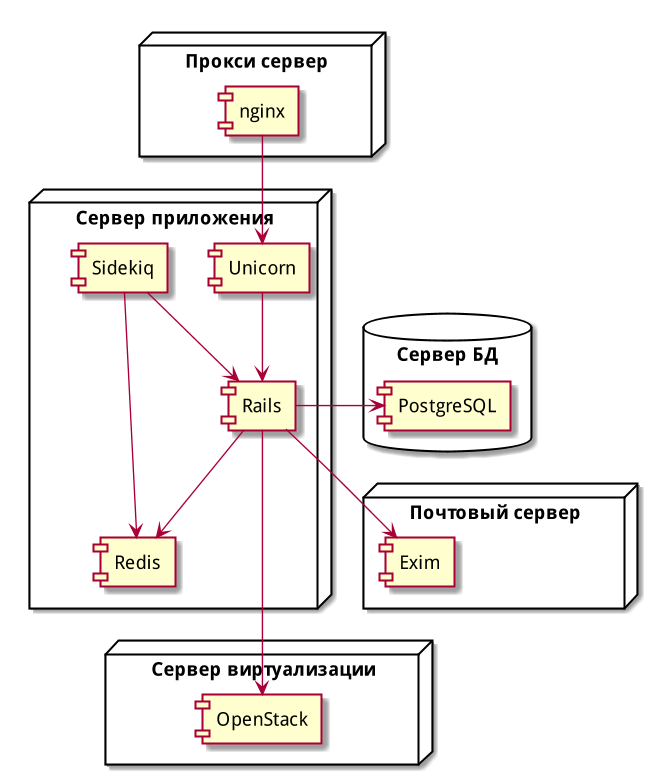
\includegraphics[scale=0.4]{umls/overview_components_diagram}
  }
  \caption{Диаграмма развёртывания.}\label{fig:overview_components_diagram}
\end{figure}

\section{Описание компонентов}\label{sec:ch4/sect2}
Приложение на Rails использут архитектуру сервисных объектов (Service Objects), которая заключается в использовании отдельных классов для инкапсуляции сложных процессов. Такие классы имеют имеют простой интерфейс, позволяющий приложению испоьзовать их как черный ящик. Экземпляры подобных классов энкапсулирует логику с данными одного определённого процесса.


Каждый компонент представляет из себя модуль с сервисными классами, которые выполняют определённую работу связанную с их компонентом.


На рисунке~\ref{fig:application_scheme} показана общая диаграмма компонентов приложения.
\begin{figure}[ht]
  \centerfloat{
    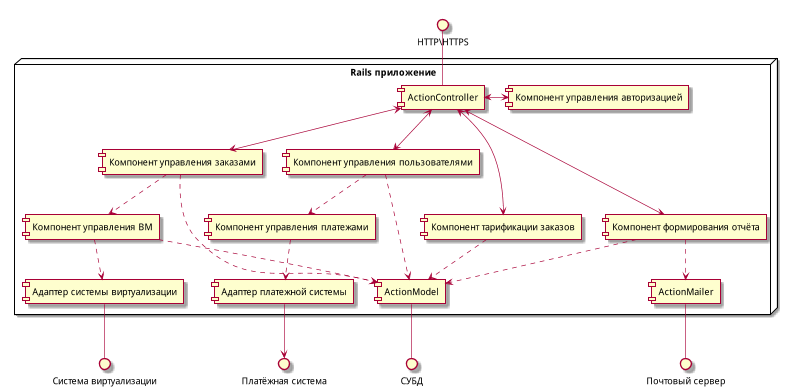
\includegraphics[scale=0.6]{umls/application_scheme}
  }
  \caption{Диаграмма компонентов приложения}\label{fig:application_scheme}
\end{figure}

\subsection{Компонент управления заказами}\label{sec:subs1}
Данный компонент, модуль, отвечает за все действия с заказами, включая проверку параметров и работы с адаптером системы виртуализации.
Каждое действие имеет свой модуль, в котором уже находятся классы для операций.

При оформлении заказа вызывается эндпоинт модуля создания заказа, который вызывает контракт проверяющий параметры, после чего сохраняет заказ в статусе "Создаётся" и отправляет сигнал разворачивания ВМ в сервис создания ВМ.

При завершении разворачивания ВМ в компонент придёт запрос на изменение состояния заказа.

На рисунке~\ref{fig:order_control_scheme} показана диаграмма компонента управления заказами.
\begin{figure}[ht]
  \centerfloat{
    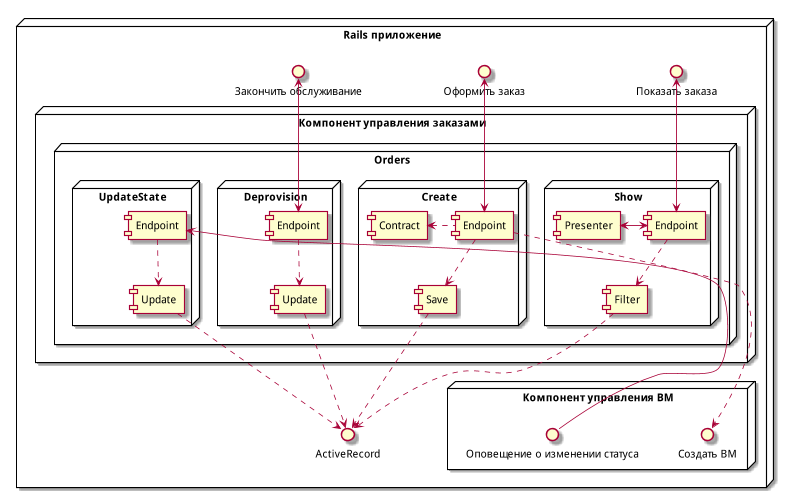
\includegraphics[scale=0.6]{umls/order_control_scheme}
  }
  \caption{Диаграмма компонента управления заказами}\label{fig:order_control_scheme}
\end{figure}

\subsection{Компонент управления ВМ}\label{sec:subs2}
Данный компонент отвечает за все действия связанные с вм, предоставляемые системой виртуализации - создание, включение, перезагрузка, выключение.

Работа компонента тесто связана с адаптером системы виртуализации, который преобразует параметры приложения в параметры системы виртуализации.

На рисунке~\ref{fig:vm_control_scheme} показана диаграмма компонента управления заказами.
\begin{figure}[ht]
  \centerfloat{
    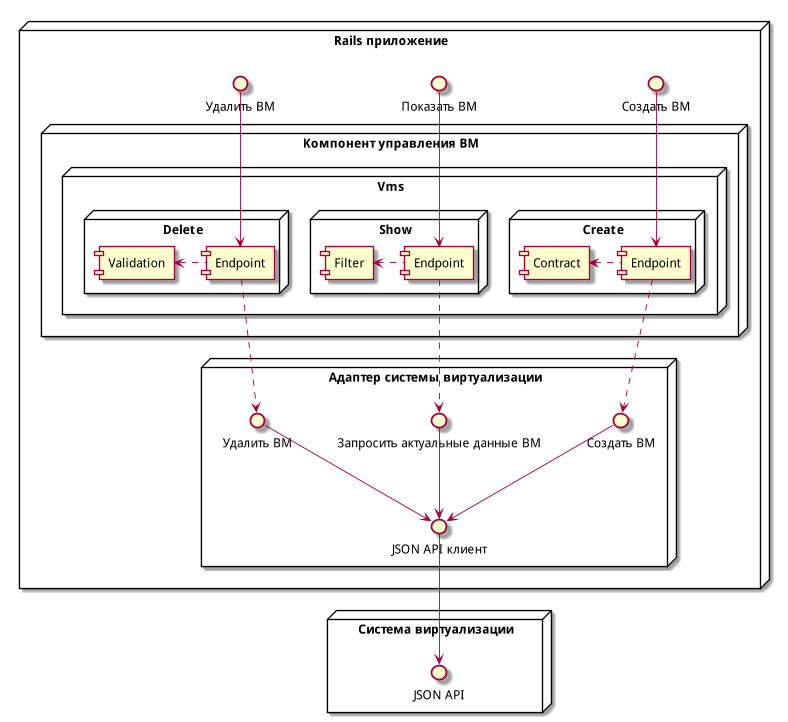
\includegraphics[scale=0.6]{umls/vm_control_scheme}
  }
  \caption{Диаграмма компонента управления ВМ}\label{fig:vm_control_scheme}
\end{figure}

\subsection{Компонент адаптера системы виртуализации}\label{sec:subs3}
Данный компонент представляет собой адаптер к системе виртуализации и отвечает непосредственную работы с системой виртуализации.

Система OpenStack разделена не сервисы отвечающие на работу с определёнными сущностями, поэтому адаптеру приходится работать с нескольми разными API разных сервисов OpenStack.

На рисунке~\ref{fig:virt_adapter_scheme} показана диаграмма адаптера.
\begin{figure}[ht]
  \centerfloat{
    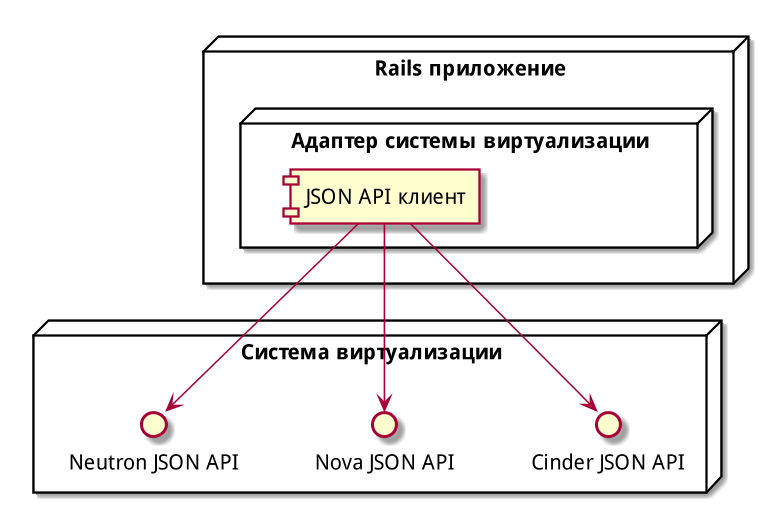
\includegraphics[scale=0.4]{umls/virt_adapter_scheme}
  }
  \caption{Диаграмма компонента адаптера системы виртуализации}\label{fig:virt_adapter_scheme}
\end{figure}

Список сервисов, с которыми адаптер имеет интеграцию:

\textbf{Nova (Compute)} - это проект OpenStack, который обеспечивает способ предоставления вычислительных экземпляров (или виртуальных серверов). Nova поддерживает создание виртуальных машин, серверов с открытым исходным кодом (с использованием сервиса Ironic) и имеет ограниченную поддержку системных контейнеров. Nova работает как набор демонов поверх существующих серверов Linux.

\textbf{Cinder (Block Storage)} - сервис, который добавляет хранилище на виртуальных машин. Блочное хранилище обеспечивает инфраструктуру для управления томами и взаимодействует с Nova (Compute) для предоставления томов для экземпляров. Служба также позволяет управлять снимками томов и их типами.

\textbf{Neutron (Networking)} - сервис позволяющий создавать и подключать к сетям интерфейсные устройства, управляемые другими службами OpenStack. Подключаемые модули могут быть реализованы для размещения различного сетевого оборудования и программного обеспечения, что обеспечивает гибкость для архитектуры и развертывания OpenStack.

\subsection{Компонент управления пользователями}\label{sec:subs4}
Компонент отвечает за все действия связанные с пользователями. Система не сохраняет данные для оплаты, но сохраняетведёт список счетов пользователя и их состояний.

На рисунке~\ref{fig:users_control_scheme} показана диаграмма компонента управления пользователями.
\begin{figure}[ht]
  \centerfloat{
    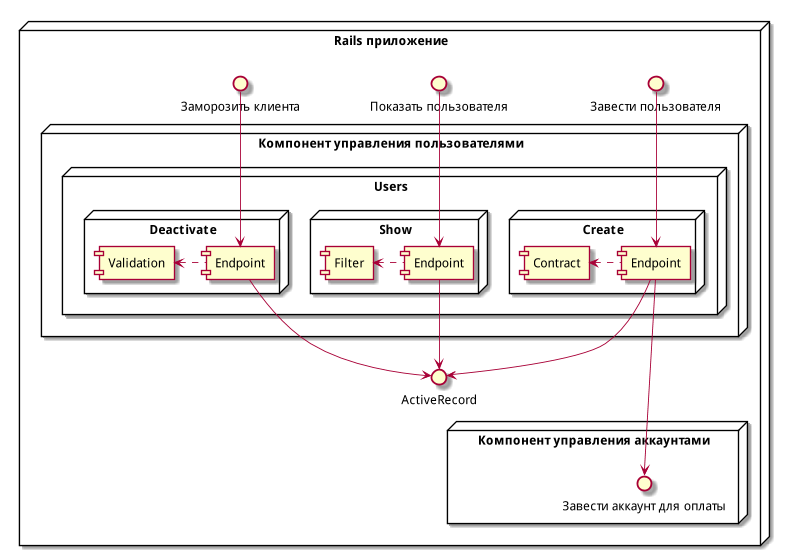
\includegraphics[scale=0.6]{umls/users_control_scheme}
  }
  \caption{Диаграмма компонента управления пользователями}\label{fig:users_control_scheme}
\end{figure}

\subsection{Компонент учета плетежей}\label{sec:subs5}
Данный компонент отвечает за управление платежами.

Основные задачи компонента:
\begin{itemize}
  \item создавать платёж в системе платёжного провайдера;
  \item следить за состоянием платежа и обновлять данные в базе на основании ответа от платёжного провайдера. 
\end{itemize}

После создания платежа и получения его данных из система платежей создаётся фоновая задача, которая периодичностью в несколько минут запрашивает у платёжной системы статус платежа. В случае его изменения данные записываются в БД.

На рисунке~\ref{fig:pay_control_scheme} показана диаграмма компонента управления платежами.
\begin{figure}[ht]
  \centerfloat{
    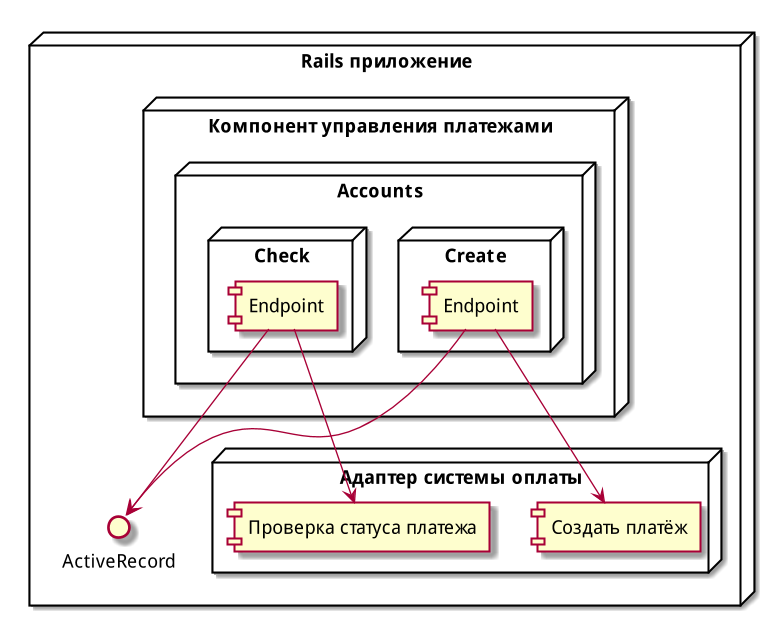
\includegraphics[scale=0.5]{umls/pay_control_scheme}
  }
  \caption{Диаграмма компонента управления платежами}\label{fig:pay_control_scheme}
\end{figure}

\subsection{Компонент управления авторизацией}\label{sec:subs6}
Для авторизации используется механизм политик. Политики представляют собой классы, каждый из которых описывает политику для определённого действия.


При запросе, в контроллере, выбирается политика для определённого в запросе действия и пользователя и проверяется возможность выполнения этого действия для пользователя.


На рисунке~\ref{fig:authorize_control_scheme} показана диаграмма компонента управления авторизацией.
\begin{figure}[ht]
  \centerfloat{
    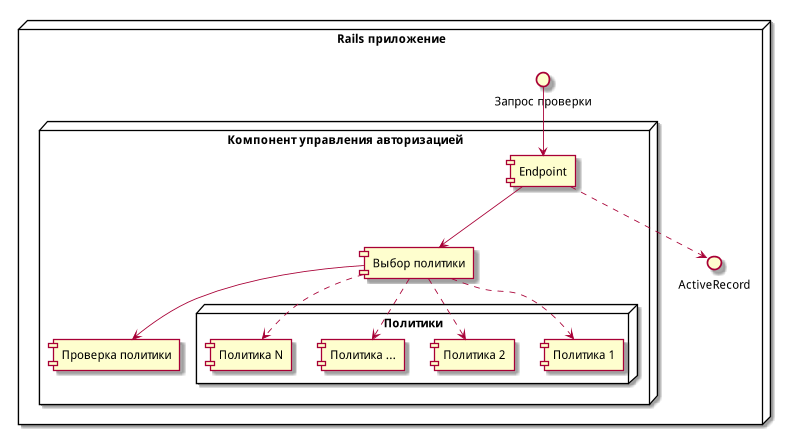
\includegraphics[scale=0.5]{umls/authorize_control_scheme}
  }
  \caption{Диаграмма компонента управления авторизацией}\label{fig:authorize_control_scheme}
\end{figure}

\subsection{Компонент адаптера платёжной системы}\label{sec:subs7}
Данный компонент представляет собой адаптер и отвечает за непосредственную работу с API системы "Яндекс.Касса".

На рисунке~\ref{fig:pay_adapter_scheme} показана диаграмма адаптера.
\begin{figure}[ht]
  \centerfloat{
    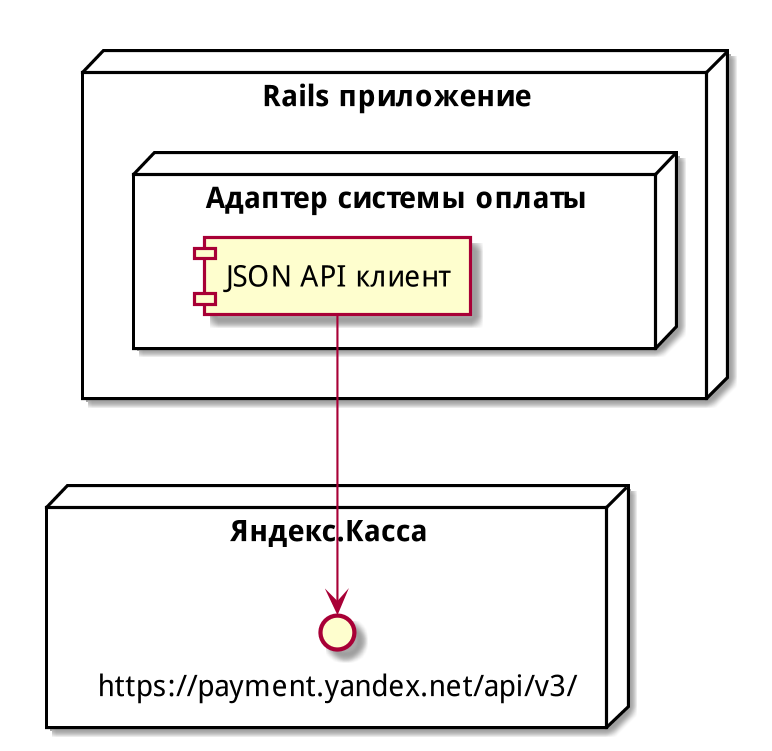
\includegraphics[scale=0.35]{umls/pay_adapter_scheme}
  }
  \caption{Диаграмма компонента адаптера платёжной системы}\label{fig:pay_adapter_scheme}
\end{figure}

\subsection{Компонент формирования отчётов}\label{sec:subs8}
Данный компонент содержит в себе логику формирования отчётов по данным, собранным при тарификации заказов.

Отчёты представляют собой файлы в формате CSV.

Отчёты формируются асинхронно и отправляются на почту запросившему их пользователю.

На рисунке~\ref{fig:report_scheme} показана диаграмма компонента формирования отчёта.
\begin{figure}[ht]
  \centerfloat{
    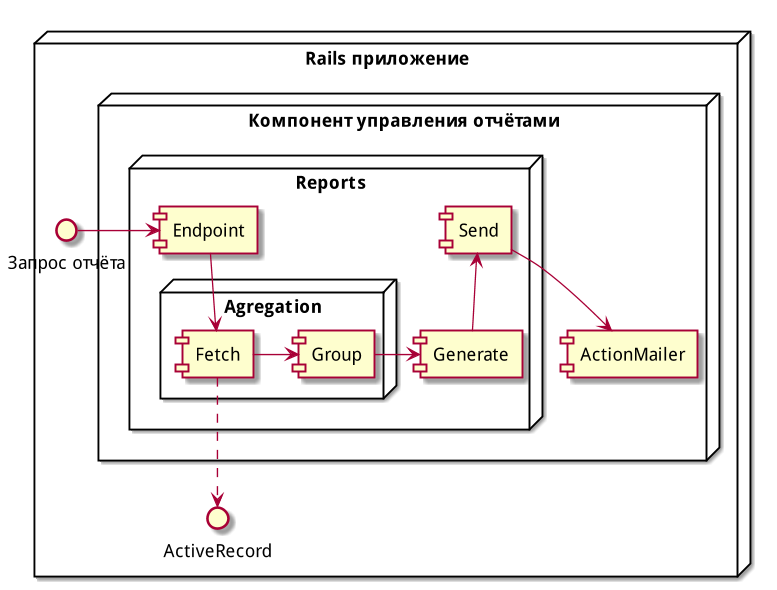
\includegraphics[scale=0.5]{umls/report_scheme}
  }
  \caption{Диаграмма компонента формирования отчёта}\label{fig:report_scheme}
\end{figure}

\subsection{Компонент тарификации заказов}\label{sec:subs9}
Данный компонент отвечает за тарификацию заказов. Заказы тарифицируются с помощью фоновой задачи, которая запускается каждый час.
Для каждого заказа сохраняется в БД <<ресурсная запись>> - запись о том, какое колчество определённого ресурса (cpu, ram, hdd) за час было потреблено заказлм с какой стоимостью и в рамках какого тарифа.

Данная схема позволяет составлять отчёты вне контекста заказов - тольпро ресурсы и конфигурации.

На рисунке~\ref{fig:tarification_scheme} показана диаграмма компонента тарификации.
\begin{figure}[ht]
  \centerfloat{
    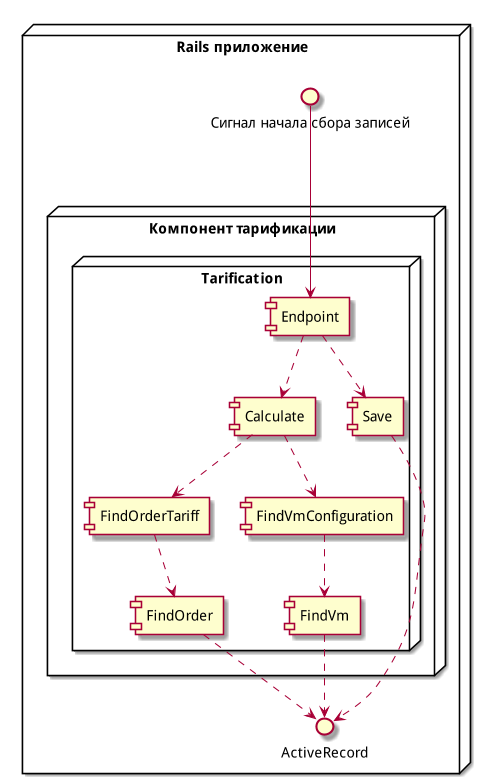
\includegraphics[scale=0.5]{umls/tarification_scheme}
  }
  \caption{Диаграмма компонента тарификации}\label{fig:tarification_scheme}
\end{figure}

\section{Концептуальная модель базы данных}\label{sec:ch4/sect3}

% \section{Компонент управления заказами}\label{sec:ch4/sect1}


% \section{Компонент управления заказами}\label{sec:ch4/sect1}
% \section{Компонент формирования отчётов}\label{sec:ch4/sect2}
% \section{Компонент работы с системой виртуализации}\label{sec:ch4/sect3}
% \section{Компонент тарификации заказов}\label{sec:ch4/sect4}

% \section{Диаграммы вариантов использования}\label{sec:ch4/sect1}
% \subsection{Создание аккаунта пользователя}\label{sec:subs12}
% \subsection{Создание заказа}\label{sec:subs13}
% \subsection{Управление заказом}\label{sec:subs14}

% \section{Диаграммы последовательностей}\label{sec:ch4/sect2}
% \subsection{Создание аккаунта пользователя}\label{sec:subs21}
% \subsection{Создание заказа}\label{sec:subs22}
% \subsection{Управление заказом}\label{sec:subs23}

% \section{Диаграмма состояний объектов системы}\label{sec:ch4/sect3}
% \subsection{Аккаунт пользователя}\label{sec:subs31}
% \subsection{Заказ}\label{sec:subs32}

% \section{Концептуальная модель базы данных}\label{sec:ch4/sect4}
% \section{Архитектура системы(?)}\label{sec:ch4/sect5}

